\begin{center}
	\includegraphics[width=\linewidth]{images/unity_desktop.png}
\end{center}

Po zalogowaniu się do systemu ujrzysz Pulpit. Widać na nim trzy elementy --- przestrzeń roboczą, wypełniającą większą część ekranu, oraz dwa panele. Panel poziomy, zwany \textcolor{ubuntu_orange}{panelem menu}, umieszczony jest u góry ekranu. Panel pionowy to \textcolor{ubuntu_orange}{Launcher} lub inaczej panel uruchamiania, zlokalizowany z lewej strony ekranu.

\subsubsection{Zmiana tła pulpitu}
Aby zmienić tło pulpitu (inaczej: tapetę), kliknij \textbf{prawym przyciskiem myszy} wolną przestrzeń roboczą i z menu kontekstowego wybierz \textcolor{ubuntu_orange}{Zmień tło pulpitu}.

\begin{wrapfigure}{r}{0.5\textwidth}
	\vspace{-10pt}	
	\begin{tikzpicture}
	\node[anchor=south west,inner sep=0] (image) at (0,0) {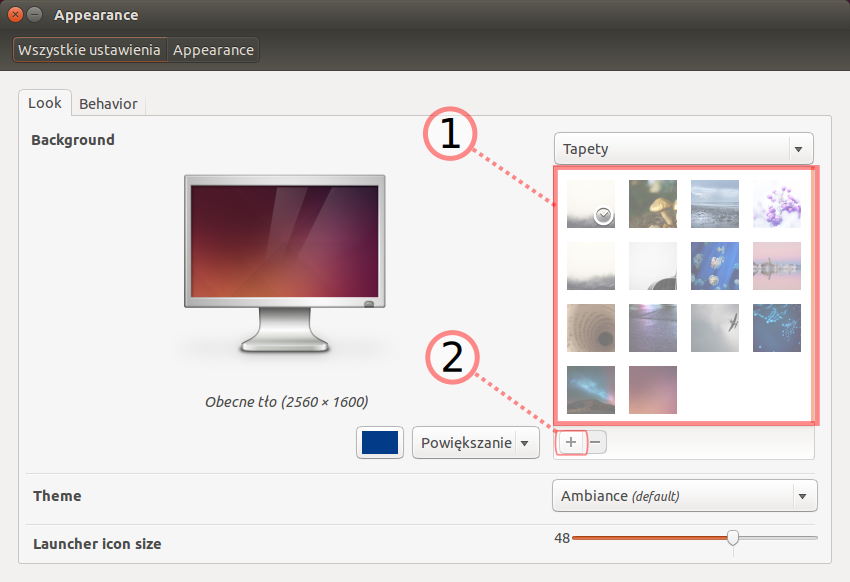
\includegraphics[width=\linewidth]{images/unity_zmiana_tapety.png}};
	\begin{scope}[x={(image.south east)},y={(image.north west)}]
		\draw[ubuntu_orange,line width=1pt,rounded corners] (0.65,0.27) rectangle (0.96,0.71);
		\draw[ubuntu_orange,line width=1pt,fill=white,fill opacity=0.75] (0.55,0.75) circle [radius=0.30cm]
			node[text=black]{\Large \textbf 1};
		\draw[ubuntu_orange,dashed,line width=1pt] (0.58,0.73) -- (0.65,0.65);
		
		\draw[ubuntu_orange,line width=1pt,rounded corners] (0.66,0.21) rectangle (0.69,0.27);
		\draw[ubuntu_orange,line width=1pt,fill=white,fill opacity=0.75] (0.55,0.35) circle [radius=0.30cm]
			node[text=black]{\Large \textbf 2};
		\draw[ubuntu_orange,dashed,line width=1pt] (0.58,0.33) -- (0.66,0.23);
    \end{scope}
\end{tikzpicture}
\end{wrapfigure}

Z listy zaznaczonej jako \circled 1 możesz wybrać którąś z dostępnych tapet. Kliknij przycisk plus \circled 2, aby otworzyć menadżer plików i wskazać inny plik graficzny na dysku twardym. Zostanie on użyty jako tapeta.

W tym oknie możesz też dokonać pewnych modyfikacji środowiska graficznego Unity. Zachęcamy do eksperymentów. Wszelkie zmiany są wprowadzane na żywo.
